% ICPE 2027, Industry Track. ACM double column (acmart, sigconf).
% Limit: 10 pages including figures and tables; references and appendices
% excluded (appendices are not published). Not anonymous. The paper must be
% marked "Industrial Paper" in its text.
%
% Page budget (sections/*.tex each say theirs at the top):
%   front matter 0.35 | 1 intro 1.15 | 2 background 0.9 | 3 TraceAssist 1.75
%   4 bench 1.25 | 5 setup 0.9 | 6 results and lessons learned 2.75
%   7 threats & open problems 0.6 | 8 conclusion 0.35          = 10.0
%
% Build: pdflatex main && bibtex main && pdflatex main && pdflatex main
\documentclass[sigconf]{acmart}

\usepackage{booktabs}
\usepackage{tabularx}
\usepackage{xspace}
\graphicspath{{figures/}}
\setlength{\emergencystretch}{1em}  % avoids lines running into the margin

\newcommand{\sysname}{TraceAssist\xspace}
\newcommand{\todo}[1]{\textcolor{red}{[TODO: #1]}}

% Filled in by ACM after acceptance.
\setcopyright{none}
\acmConference[ICPE '27]{ACM/SPEC International Conference on Performance Engineering}{May 24--28, 2027}{Gothenburg, Sweden}
\acmYear{2027}
\acmDOI{}
\acmISBN{}
\settopmatter{printacmref=false}

\title{TraceAssist: Answering Kernel Trace Questions in Natural Language}
\subtitle{Industrial Paper}

\author{Sneh Patel}
\affiliation{%
  \institution{Brock University}
  \city{St.\ Catharines}
  \state{Ontario}
  \country{Canada}}
\email{sp18oo@brocku.ca}

\author{Yuvraj Sehgal}
\affiliation{%
  \institution{Brock University}
  \city{St.\ Catharines}
  \state{Ontario}
  \country{Canada}}
\email{ys19rk@brocku.ca}

\author{Mahsa Panahandeh}
\orcid{0000-0002-6369-8982}
\affiliation{%
  \institution{University of Ottawa}
  \city{Ottawa}
  \state{Ontario}
  \country{Canada}}
\email{mpanahan@uottawa.ca}

\author{Naser Ezzati-Jivan}
\orcid{0000-0003-1435-6297}
\affiliation{%
  \institution{Brock University}
  \city{St.\ Catharines}
  \state{Ontario}
  \country{Canada}}
\email{nezzatijivan@brocku.ca}

\renewcommand{\shortauthors}{Patel et al.}


\begin{document}

\begin{abstract}
% Abstract (part of the 0.35-page front matter)
Large language models (LLMs) cannot read execution traces, which are far larger than their context windows and describe executions absent from their training data, and when they answer anyway they can report problems that are not there. We present \sysname, an assistant developed for Ciena that answers natural-language questions about Linux kernel traces. Analyzers built on Trace Compass compute measured findings from the whole trace; small LLM decisions, checked by code, map a question to the threads it concerns; and an LLM writes the answer from the findings alone. \sysname is part of Trace Compass: each answer names, and opens, the Trace Compass views that show its evidence. To measure false alarms as well as answers, we built a symptom bench: nine C programs with 44 injectable faults covering 48 performance symptoms, 56 LTTng traces with program-written answer keys, and 516 yes/no answers per system to questions asked of traces with and without each symptom. With the same answering model, \sysname reaches a balanced accuracy of 0.93 (precision 0.85, recall 0.93), stable across three runs, against 0.58 for baselines that read trace text with or without retrieved documentation, 0.69 for an LLM given TMLL's analyses, and 0.79 for a coding agent with a shell over the whole trace, which raised nearly five times as many false alarms and took 13 times as long per answer (median). We report the lessons of developing against such a bench and the problems that remain open.

\end{abstract}

\ccsdesc[500]{Software and its engineering~Software performance}
\ccsdesc[300]{Software and its engineering~Software testing and debugging}
\ccsdesc[300]{Computing methodologies~Natural language processing}
\keywords{execution traces, LTTng, Trace Compass, large language models,
retrieval-augmented generation, performance diagnosis}

\maketitle

% 1 Introduction -- 1.15 pages
\section{Introduction}
\label{sec:intro}

Large language models (LLMs) now sit inside search engines, editors and developer tools. They are reliable for knowledge that is common on the web, but struggle with information that is too large to process, where accuracy can drop even before the context limit is reached~\cite{liu2024lost}, and with rare or private information, such as a company's internal systems, that is poorly represented in their training data~\cite{kandpal2023longtail}. In both cases they can fill the gaps with convincing but unsupported claims~\cite{ji2023hallucination}.

Execution traces combine both problems. A kernel tracer such as LTTng~\cite{desnoyers2006lttng} records every system call, scheduling decision and interrupt; 30 seconds of a small program on a desktop yields millions of events, about 66 tokens each as text, far beyond any context window. And a developer's question, such as \emph{why one thread is slow}, concerns one specific execution that appears in no training corpus. Tools such as Trace Compass~\cite{tracecompass} can answer it, but require expertise in kernel scheduling and in the tool's many views. Retrieval-augmented generation (RAG)~\cite{lewis2020rag} can add documentation, which explains what a \texttt{futex} wait is but not how long a thread waited or which thread woke it.

\textbf{Industrial context.} \sysname was developed for Ciena, whose engineers analyze execution traces often. Answering even a simple question about a trace, such as \emph{why is this run slow?}, can take an engineer hours of work in Trace Compass's views; \sysname answers such a question in under two minutes (a median of 17\,s per answer on our bench). Two requirements followed. First, answers must come from the whole trace, with measured values an engineer can check in Trace Compass. Second, the assistant must not invent problems: an engineer who chases a false alarm in a large system loses hours, and stops trusting the tool.

\sysname answers natural-language questions about Linux kernel traces by letting Trace Compass compute the evidence. Analyzers built on its kernel analyses produce measured \emph{findings}, such as how a thread's time divides between running, waiting for a CPU and being blocked, which thread ended each wait, or which waits never ended. Small LLM decisions, checked by code, map a question to the threads it means; statistical probes and retrieved documentation add context; and an LLM writes the answer from the findings alone. It is part of Trace Compass, and every answer opens the Trace Compass views that show its evidence, so the engineer can check it.

An earlier prototype answered all 13 questions correctly about one program with one lock bug. That evaluation could not show the failure that matters most in practice, a claim that a problem exists when it does not, because every question had a real answer. We therefore built a \emph{symptom bench}: nine C programs whose fault switch injects one of 44 faults, or none, covering 48 symptoms engineers ask about. The 56 traces come with answer keys written by the programs themselves, and each question is asked both of traces with its symptom and of traces without it, in a precise and an everyday wording. We use the bench to answer five research questions:
\textbf{RQ1} How accurately does \sysname detect the bench's symptoms, compared with four baselines?
\textbf{RQ2} How often does each system report a problem that is not there, or decline to answer?
\textbf{RQ3} Which symptoms, question types and wordings does each system get wrong?
\textbf{RQ4} How consistent are \sysname's verdicts when the same question is asked again?
\textbf{RQ5} What does an answer cost in time and money?

On the bench's 516 answers per system, \sysname reaches a balanced accuracy of 0.93 (precision 0.85, recall 0.93), stable across three runs ($\pm$0.005). With the same answering model, baselines that read trace text, alone or with retrieved documentation, reach 0.58 and mostly decline to answer; a baseline given Trace Compass's standard analyses through TMLL~\cite{shahedi2025tmll} reaches 0.69; and a coding agent with the whole trace and a shell reaches 0.79, with 113 false alarms against \sysname's 24 and 13 times its median time per answer.

Our contributions are:
\begin{itemize}
  \item \sysname, an assistant that grounds every statement in findings computed by Trace Compass from the whole trace, and its integration into Trace Compass (Section~\ref{sec:traceassist}).
  \item A symptom bench of nine fault-switch programs, 56 traces with program-written answer keys, and 112 question wordings over 258 question--trace pairs, which measures false positives as well as answers (Section~\ref{sec:bench}).
  \item A comparison with four baselines that use the same answering model, including a coding agent (Sections~\ref{sec:setup}--\ref{sec:results}).
  \item Lessons from developing an LLM assistant against such a bench, and the open problems that remain (Sections~\ref{sec:lessons} and~\ref{sec:threats}).
\end{itemize}

% 2 Background and related work -- 0.9 page
\section{Background and Related Work}

\subsection{Kernel Tracing with LTTng and Trace Compass}

LTTng~\cite{desnoyers2006lttng} records Linux kernel events with low overhead: system call entries and exits, scheduler switches and wake-ups, timers, interrupts, and block-device, network and signal events; Gebai and Dagenais~\cite{gebai2018survey} survey the Linux kernel and user-space tracers and their overhead, and kernel-level events have been shown to enrich empirical performance research~\cite{noferesti2024kernel}. Trace Compass~\cite{tracecompass} turns these events into \emph{state systems}, time-indexed models of each thread's state, current system call and each CPU's run queue, and into an \emph{execution graph} of which thread woke which. The \emph{critical path} of a thread follows this graph backwards through its waits to the work that delayed it~\cite{giraldeau2016wait}. Critical paths also profile latency at scale in distributed services~\cite{eaton2022cpt,zhang2022crisp}, and Trace Compass's critical path has been used to detect anomalies with an LSTM at a fraction of the cost of system-call features~\cite{nourollahi2025tracelens} and to find performance archetypes and regressions~\cite{shahedi2026archetypes}. These analyses are shown in views such as Control Flow, Resources and Critical Path. The headless Trace Compass Trace Server exposes the same analyses through the Trace Server Protocol~\cite{tsp}, which TMLL uses. Reading these views well requires knowing what each thread state means and where to look, which is the expertise \sysname aims to supply.

\subsection{Related Work}

\textbf{Language models over traces.} TAAF~\cite{ezaz2026taaf} answers natural-language questions about LTTng kernel traces by building a time-indexed Trace Compass state system and, for each question, extracting a knowledge graph of threads, CPUs and resources over which an LLM reasons. On TraceQA-100, 100 questions about slices of a SciMark~2.0 trace, it improves accuracy by up to 31.2\% over the state system's numeric output, mostly on multi-hop and causal questions; our hub-scope labels follow its distinction between single- and multi-hop questions. \sysname differs in three ways. Its analyzers compute the measurements an answer needs, such as wait chains, per-round finish times and stuck waits, so the LLM explains results rather than deriving them from a graph. It analyzes whole traces rather than slices. And our evaluation asks each question of traces with and without the symptom, so it measures false positives.

\textbf{Machine learning for Trace Compass.} TMLL~\cite{shahedi2025tmll}, built with Ericsson, applies anomaly detection, change-point detection, correlation and capacity planning to the Trace Server's analyses. Its authors report that technical excellence alone did not drive adoption by practitioners; explainable results and expert knowledge built into the interface did. \sysname uses TMLL as one source of supporting evidence, and we evaluate TMLL's analyses, given to an LLM, as a baseline.

\textbf{Deterministic evidence with LLM explanation.} Outside kernel tracing, two systems share \sysname's division of labour. RCACopilot~\cite{chen2024rcacopilot} matches each cloud incident at Microsoft to a handler that collects diagnostic data, then has an LLM predict the root-cause category and explain it, reaching an accuracy of up to 0.766 on a year of incidents. Opal~\cite{zaeed2025opal} adds hardware-counter and Roofline analytics to LLM prompts to optimize GPU kernels; even a single source of insight produced a speedup in over 98.5\% of 1{,}640 experiments, and its one incorrect result stemmed from a vague diagnostic, which supports giving the LLM precise findings. LLMs have also been fine-tuned to recommend root causes and mitigations for over 40{,}000 cloud incidents~\cite{ahmed2023recommending}, and Praxium diagnoses cloud anomalies from telemetry and service dependencies~\cite{kumar2026praxium}. Closer to kernel traces, Fournier et al.~\cite{fournier2021cause} find the causes of slow web requests by clustering and comparing their kernel-level executions. \sysname brings the division of labour to kernel traces, where the evidence must first be computed from millions of events, and to open questions rather than classification or code generation.

\textbf{Coding agents.} General coding agents such as Codex~\cite{codexcli} interleave reasoning with tool use~\cite{yao2023react} and are evaluated mostly on resolving code issues~\cite{jimenez2024swebench}; given a shell, they can run tools over a trace and compute their own evidence. We include one as a baseline: it shows what an engineer gets today without a trace-specific assistant, and at what cost.

% 3 TraceAssist -- 1.75 pages (incl. Fig. 1, full width)
\section{TraceAssist}
\label{sec:traceassist}

\begin{figure*}[t]
\centering
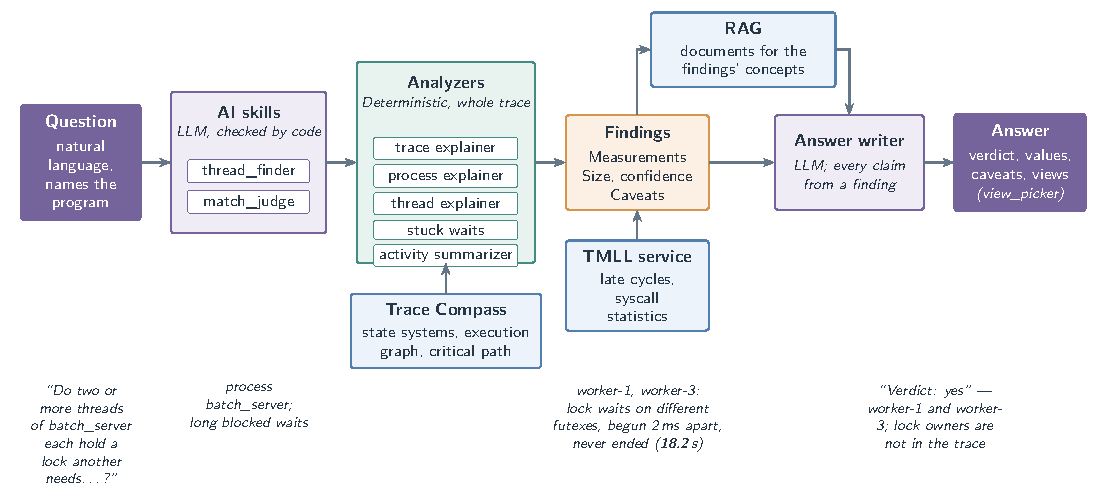
\includegraphics[width=\textwidth]{traceassist_pipeline}
\Description{Flow diagram: question, AI skills, analyzers over Trace Compass, findings with TMLL and RAG, answer writer, answer; with a deadlock question traced through each step.}
\caption{\sysname's pipeline from question to answer. Code computes every fact about the trace; the LLM makes small, checked decisions (the AI skills) and writes the answer from the findings. The italic text follows one bench question, on a trace where two of \texttt{batch\_server}'s workers deadlock, through the steps (Section~\ref{sec:results}).}
\label{fig:pipeline}
\end{figure*}

\sysname follows one rule: \emph{code computes every fact about the trace, and the LLM only makes small, checked decisions and writes the answer from those facts}. A 30-second trace of a small program on a desktop holds 1.4--25 million events (Section~\ref{sec:bench}); the LLM never reads them. It receives about 10--30 thousand tokens of computed evidence per question. Fig.~\ref{fig:pipeline} shows the parts, which we describe in the order a question passes through them; Fig.~\ref{fig:arch} shows the full architecture, drawn on TMLL's architecture figure~\cite{shahedi2025tmll}, with the components we added marked NEW.

\begin{figure*}[t]
\centering
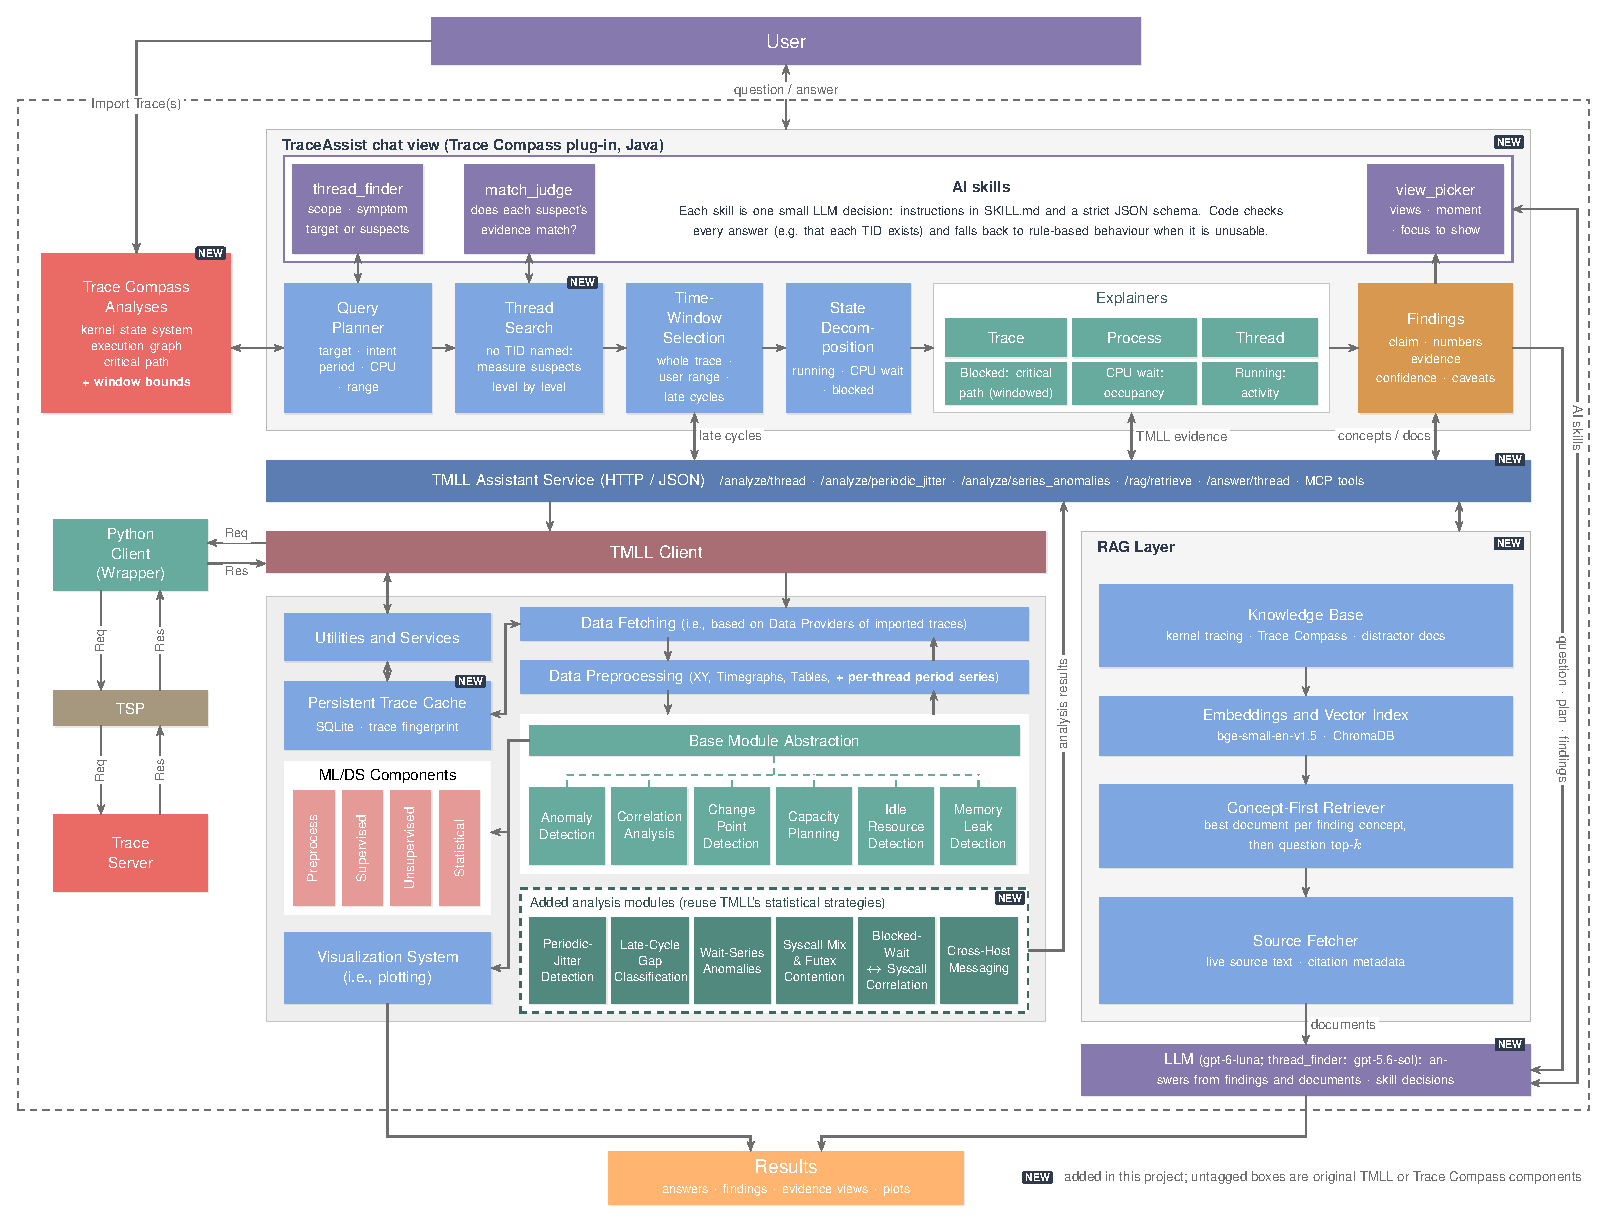
\includegraphics[width=\textwidth]{architecture}
\Description{Architecture diagram of TraceAssist inside Trace Compass, the TMLL assistant service and client with added analysis modules, the RAG layer and the LLM, with new components marked.}
\caption{\sysname's architecture, drawn on TMLL's architecture figure. Boxes marked NEW were added in this work; the others are original TMLL or Trace Compass components. The AI skills (top row) and the LLM are the only calls to a language model; code checks every skill's answer.}
\label{fig:arch}
\end{figure*}

\subsection{From Question to Target}

Users rarely know thread IDs. They ask \emph{``Is something in batch\_server holding a lock too long?''} The first step decides what the question is about: one thread, a process, or the whole trace; what it asks (explain a thread's time, find a process's bottleneck, find late cycles); and the time window. This step needs language understanding most, so it is handed to the first of three \emph{AI skills}.

An AI skill is one narrow decision delegated to an LLM, defined by an instruction file and a strict JSON schema, and checked by code before use:
\begin{itemize}
  \item \textbf{thread\_finder} reads the question and an inventory of the trace's processes and threads, and returns the scope, the symptom the question describes (e.g., a one-off delay or a bottleneck), and either the target or up to five suspects. Every TID and PID it names must exist in the trace; if the call fails, a rule-based planner takes over.
  \item \textbf{match\_judge} rates suspects during the \emph{thread search}. When the target is unclear, code measures every suspect one level deeper at a time (time by state, then the symptom's detail, then the worst moment), and after each level the skill rates whether each suspect's measured evidence matches the question. Code turns the ratings into a pick with a percentage and a confidence label, which the answer reports.
  \item \textbf{view\_picker} chooses the 1--3 Trace Compass views that show the answer's evidence, the moment to show, and what to select in each, from one description file per view. Code computes the zoom range.
\end{itemize}
Skills can be read and changed without touching the Java code. In normal use their decisions are cached per input, so a repeated question gets the same target.

\subsection{Analyzers and Findings}

The analyzers are Java code inside Trace Compass. They read its kernel analyses: the \emph{state system}, which holds each thread's state, current system call and each CPU's run queue over time, and the \emph{execution graph}, which records which thread woke which. There is one analyzer per kind of target:
\begin{itemize}
  \item The \emph{trace explainer} summarizes what was recorded: which events, which processes ran and used the CPU, and which process is the workload rather than background activity or the tracer.
  \item The \emph{process explainer} splits each thread's time into running, waiting for a CPU and blocked; follows the execution graph's wake-up edges to find which thread ended each wait; and names the \emph{bottleneck}, the thread the main thread waits on, with its wait chain to the root. Over every round it measures when each thread finishes and how much faster rounds would be without the bottleneck's wait.
  \item The \emph{thread explainer} splits one thread's time by state and explains each large share: for blocked time, the system call and the critical path~\cite{giraldeau2016wait} of the longest wait; for CPU waits, which threads held the CPU; for running time, user versus kernel time.
\end{itemize}
Trace Compass computes a critical path over a thread's whole life; we added an optional time window so that it can cover one wait, such as the longest. This is the only change to Trace Compass itself.

Two further components cover what the state system does not keep; the first was added, and the second extended, when the evaluation exposed gaps (Section~\ref{sec:lessons}). \emph{Stuck-wait detection} reports threads still blocked at the end of the trace, which the execution graph omits because they are never woken, and classifies their system calls as sleeps, timed waits or waits that only another thread can end; several lock-style waits beginning together are reported, hedged, as consistent with a deadlock. The \emph{activity summarizer} reads every event once and records what the state system does not keep: which file, socket or pipe each call used, open modes, syncs and their durations, threads and processes created and how they ended, and each thread's time in system calls by what they wait on (storage, network, futex, sleep, and so on).

Every result is a \emph{finding}: a JSON object with a one-sentence claim whose numbers are filled in by code, the window it covers, the evidence, a confidence level and caveats. Inferences a kernel trace cannot observe directly, such as which thread holds a lock, are marked medium confidence. Findings also carry their \emph{size}: a bottleneck's impact on the round is labelled negligible (under 5\%), minor or significant (25\% or more), and scheduling delays are counted by length. In a healthy program some thread always finishes last and some wait is always the longest; without sizes, the answer writer reported those as problems.

\subsection{Statistical Evidence and Documentation}

\textbf{TMLL and our modules.} TMLL~\cite{shahedi2025tmll} is the Trace Compass project's machine-learning library. It fetches the Trace Server's analyses through the Trace Server Protocol and applies ready-made modules, such as anomaly detection, change points, correlation, idle resources, capacity planning and memory leaks, to system-wide series such as CPU, memory and disk usage. We keep the library unchanged and built our own components on it (marked NEW in Fig.~\ref{fig:arch}). They analyze one thread's series rather than the whole system, reusing TMLL's statistical strategies:
\begin{itemize}
  \item a \emph{system-call frequency} module, which counts each thread's calls by name and category, classifies the dominant kind (file I/O, synchronization, networking, and so on), and measures futex contention;
  \item per-thread \emph{anomaly detection}: periodic-jitter detection over the intervals between a thread's wake-ups, which finds its late cycles with TMLL's z-score strategy; classification of what the thread was doing during each late cycle; and a wait-series detector that tells a constant slowdown, where every round waits alike, from occasional spikes;
  \item correlation of long blocked waits with the system calls that overlapped them, and detection of messages between hosts.
\end{itemize}
A local HTTP service exposes these to the Java analyzers, and a persistent cache keyed by the trace's fingerprint scans each trace's tables once. We also fixed TMLL's z-score preprocessing, which dropped every value tied at the minimum and so found nothing on a very regular periodic thread. Results return as findings. The service is optional: when it fails, \sysname records an ``unavailable'' finding and the analyzers' findings are unchanged.

\textbf{RAG.} The knowledge base holds 37 Markdown documents: 15 on Linux kernel tracing concepts (futex waits, thread states, wake-ups, system calls), 12 on Trace Compass analyses and their limits, and 10 on Django from an unrelated workload. Documents are embedded with \texttt{bge-small-en-v1.5}~\cite{xiao2023cpack} and stored in ChromaDB. Retrieval is driven by the findings: each concept a finding names, such as the system call a thread blocked in, retrieves its best document, and the question's own search fills the remaining places, six in all. Documents explain concepts; they are never a source of facts about the trace.

\subsection{Answer Writer}

One LLM call writes the answer from a JSON object holding the question, the plan, the findings and the documents. Its rules require that every statement about the trace come from a finding, with its numbers; that no cause, thread or duration be added that no finding states; that missing evidence be stated rather than guessed; that medium-confidence findings be presented as likely; and that a question of the form ``is X happening?'' be decided by the size of the evidence against the question's threshold, so that a minor bottleneck or a handful of delays among thousands does not count. The answer starts with the target the thread search picked, if any, and ends with the views to open.

All LLM calls use OpenAI's \texttt{gpt-6-luna}, except thread\_finder, which uses the larger \texttt{gpt-5.6-sol} at temperature~0. Choosing the threads a question means is the most complex decision in the pipeline, and on a smaller question set used in development, the smaller \texttt{gpt-5.6-luna} picked the wrong threads too often.

\subsection{Integration in Trace Compass}
\label{sec:deployment}

\begin{figure*}[t]
\centering
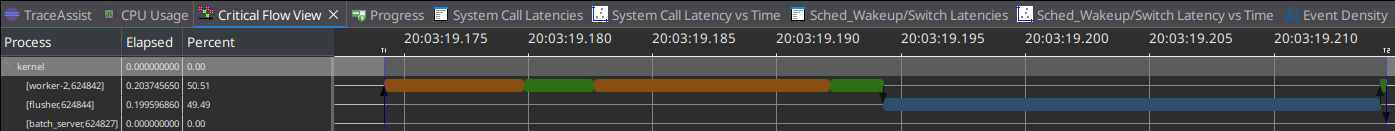
\includegraphics[width=\textwidth]{critical_path_holder_sleeps}
\Description{Screenshot of Trace Compass's critical path view: worker-2 alternates between waiting for a CPU and running, then flusher sleeps on a timer for about 20 ms before worker-2 finishes.}
\caption{The Critical Path view that \sysname opened for \emph{``What is batch\_server's main thread waiting on in each round, and what is holding that up?''} on the bench's lock-holder-sleeps trace, zoomed to one typical 40.3\,ms round. The main thread's wait runs through \texttt{worker-2} (orange: waiting for a CPU while the other workers run; green: running) and then \texttt{flusher}, asleep on a timer (blue) for 19.9\,ms while holding the lock \texttt{worker-2} needs. The answer reported this chain with per-round values within 0.1\,ms of the program's own measurements: \texttt{worker-2} blocked 23.17\,ms per round (measured 23.18\,ms), the lock held 40.13\,ms (40.12\,ms), over all 484 rounds.}
\label{fig:critpath}
\end{figure*}

\textbf{Answers that point to their evidence.} An engineer should not have to trust the answer. Every answer ends with the Trace Compass views that show its evidence, chosen by view\_picker: which views, which moment (the worst wait, a typical round, a late cycle, or the whole trace), what to select in each, and what to look for (Fig.~\ref{fig:critpath}). \sysname then opens these views itself, zoomed to that moment, including a Critical Path computed for the wait in question. The engineer checks the claim in the standard view they already know, and continues the analysis from there.

\sysname is a Trace Compass plug-in: questions are asked in a chat view next to the trace, and the answer streams into it. The pipeline itself has no user interface, so the same code also runs headless in the Trace Compass Trace Server; the evaluation asks its questions there. On 60 test questions, the two chose identical targets and findings.

\textbf{Implementation.} \sysname is about 16{,}600 lines of Java in one Trace Compass plug-in, about 3{,}800 lines of Python for the TMLL modules and the RAG layer, three skill files and 13 view descriptions. The only change to Trace Compass is the critical-path time window. The bench adds about 2{,}100 lines of C for the nine programs and 1{,}700 lines of Python and shell to record the traces, generate the questions and pairs, and score the answers.

% 4 The symptom bench -- 1.25 pages (incl. Table 1)
\section{The Symptom Bench}
\label{sec:bench}

A question whose answer is always ``yes'' cannot reveal a tool that reports problems that are not there. The bench therefore pairs every fault with a \emph{negative control}: the same program run healthy, or with a different fault, under the same background activity. Asking the same question of both traces measures true and false positives and negatives.

\subsection{Symptoms, Programs and Faults}

We collected 48 performance symptoms that engineers ask about, in seven groups: \emph{timing} (7, e.g., a one-off delay, jitter, tail latency), \emph{waiting} (12, e.g., a bottleneck thread, deadlock, lock contention, priority inversion, waiting on disk or the network), \emph{CPU} (11, e.g., a CPU hog, scheduling delay, load imbalance, interrupt storm), \emph{system calls and I/O} (7, e.g., slow calls, polling, file churn), \emph{lifecycle} (4, e.g., crash, thread churn), \emph{pipelines} (4, e.g., the slowest stage, thundering herd), and \emph{unexpected} behaviour (3). Each has a written criterion for ``present''.

We wrote nine C programs, each one workload with a \texttt{-{}-fault} switch (Table~\ref{tab:programs}). \texttt{-{}-fault none} is the healthy run; every other value injects one problem. The 44 faults and 9 healthy runs make 53 scenarios that cover all 48 symptoms. The faults are real behaviour, not simulated events: the interrupt storm, for example, has a thread issue small direct disk reads from the victim's CPU, whose NVMe completion interrupts take about 22\% of that CPU for 12\,s.

\begin{table}[t]
\centering
\caption{The nine bench programs and their faults. Each also has a healthy run.}
\label{tab:programs}
\footnotesize
\setlength{\tabcolsep}{3pt}
\begin{tabularx}{\columnwidth}{@{}>{\raggedright\arraybackslash}p{1.45cm}>{\raggedright\arraybackslash}X@{}}
\toprule
Program & Workload; faults \\
\midrule
\texttt{batch\_server} & Coordinator hands work to 4 workers per round; lock holder sleeps, contention, convoy, deadlock, hang, priority inversion \\
\texttt{ticker} & Sampler that must run every 2\,ms; one-off delay, jitter, gradual slowdown, sudden change, oversleeping, real-time preemption \\
\texttt{crunch} & 8 compute threads meeting at a barrier; load imbalance, barrier straggler, CPU hog, busy-wait, CPU starvation, oversubscription, migrations, odd worker \\
\texttt{filestore} & Record store with writer, reader, stats threads; disk wait, small calls, polling, retry loop, file churn, unexpected scan \\
\texttt{pipeline} & Reader $\rightarrow$ parser $\rightarrow$ 4 sinks over bounded queues; slow stage, bursty input, thundering herd, idle workers, idle thread \\
\texttt{kvstore} & 4 clients and a server process over loopback TCP; slow backend, tail latency, network wait \\
\texttt{cachesvc} & In-memory cache with a loader and 2 servers; memory pressure, allocation churn \\
\texttt{jobrunner} & Dispatcher with a pool of 4 job threads; slow start-up, slow shutdown, crash, fork storm, thread churn, never exits \\
\texttt{reporter} & Renders a report every 50\,ms; noisy neighbour process, interrupt storm \\
\bottomrule
\end{tabularx}
\end{table}

\textbf{Keeping the trace the only evidence.} Thread, process and file names never name the fault, and every trace gets a random name. CPU work is a calibrated arithmetic loop, so a busy thread leaves no misleading system calls. Threads that wake each other share a CPU, avoiding a known misattribution of cross-CPU wake-ups in Trace Compass's critical path. Runs that stay stuck (deadlock, hang, never exits) are ended by a watchdog only after tracing has stopped.

\subsection{Traces and Ground Truth}

Each scenario was recorded for 30\,s with LTTng kernel tracing of the whole machine: scheduling, system calls, timers (including high-resolution timer starts and cancels), interrupts, and network, block-device and signal events. Three scenarios were recorded again \emph{without} the events their symptom depends on (a crash without signal events, a disk wait without block events, a network wait without network events), where the correct answer is that the trace cannot show it. The 56 traces hold 1.4--25.3 million events each (159 million in all, 5\,GB), with no events discarded. Every trace also contains the desktop's own activity, so ``absent'' is reliable only for the program itself, and every graded question names its program.

Each program writes its own answer key while it runs, through a pipe rather than a file the trace could record: the symptoms its fault makes \emph{present}; those arguably present as a side effect, marked \emph{don't care} and not graded; every thread with its ID; when the fault acts; and the program's own measurements, such as round times and lock waits. Every other symptom is \emph{absent}.

Vague words need thresholds. A healthy thread is sometimes delayed by a millisecond, and a healthy writer's \texttt{fdatasync} takes 2\,ms, so without a threshold ``yes'' is defensible on a healthy trace. We measured each symptom on every trace of its program and chose thresholds that separate the faults from the healthy runs, such as ``kept waiting to run for 1\,ms or more at least 50 times, or 10\,ms or more once''.

\subsection{Questions and Pairs}

\begin{table*}[t]
\centering
\caption{One bench question per category, in its two wordings, with the symptom, program and hub scope it tests.}
\label{tab:questions}
\footnotesize
\setlength{\tabcolsep}{4pt}
\begin{tabularx}{\textwidth}{@{}>{\raggedright\arraybackslash}p{2.1cm}>{\raggedright\arraybackslash}X>{\raggedright\arraybackslash}p{5.2cm}@{}}
\toprule
Category (symptom, program, hub) & Precise wording & Everyday wording \\
\midrule
Comprehension (crash, \texttt{jobrunner}, single) & Does any process of jobrunner die from a signal (such as a segfault or an abort) instead of exiting normally? If so, which process, and which signal? & Did anything in jobrunner crash or get killed? What was it? \\
Root cause (noisy neighbour, \texttt{reporter}, multi) & Does another process compete with reporter for its CPU and slow its work down by 25\% or more? If so, which process, and how much does reporter lose? & Is another program slowing reporter down? Which one, and by how much? \\
Dependency (deadlock, \texttt{batch\_server}, multi) & Do two or more threads of batch\_server each hold a lock that another of them needs, so that they stay blocked for good? If so, which threads? & Are any threads in batch\_server waiting on each other forever? Which ones? \\
Quantitative (one-off delay, \texttt{ticker}, single) & Does any cycle of ticker's sampler thread take far longer than usual (at least 5 times its normal length)? If so, when did it happen, and how late was it? & Did ticker's sampler hiccup once, with one cycle much later than all the others? When, and by how much? \\
Remediation (small calls, \texttt{filestore}, single) & Does filestore make tens of thousands of tiny system calls per second where a few larger ones would do? If so, which calls, and what change would fix it? & Is filestore making thousands of tiny reads or writes? How should it be changed? \\
\bottomrule
\end{tabularx}
\end{table*}


There is one question per symptom and program that can show it: 56 questions. Each has a category, as in our prototype study (comprehension, root cause, dependency, quantitative, remediation), and a hub scope~\cite{ezaz2026taaf}: \emph{single-hub} questions concern one thread or process, \emph{multi-hub} ones combine evidence across several. Every question is written in two wordings, both naming the program. The \emph{precise} wording states exactly what counts, with a threshold where the symptom has a size; the \emph{everyday} wording keeps a user's vagueness (Table~\ref{tab:questions}). A remediation question first asks whether the problem exists, so on a trace without it the right answer is that there is nothing to fix. A question names only threads present in every trace of its program, so a name never reveals a fault.

Each question is asked of up to five traces of its program: every trace where its symptom is present or cannot be seen, the healthy run, then the program's other faults, picked at random with a fixed seed. This gives 258 question--trace pairs: 74 where the symptom is present, 178 where it is absent, and 6 where the trace cannot show it (events that were not recorded, including page faults for memory pressure, and busy-waiting, which a kernel trace cannot tell apart from computing). With both wordings, each system gives 516 answers.

Every system receives the same instruction after every question: \emph{``Begin your answer with exactly one line: `Verdict: yes', `Verdict: no', or `Verdict: cannot tell from this trace'. Then answer the question.''} Code reads the verdict, so the counts of true and false positives and negatives need no judge.

% 5 Experimental setup -- 0.9 page
\section{Experimental Setup}
\label{sec:setup}

We compare \sysname with four baselines on the bench to answer RQ1--RQ5 (Section~\ref{sec:intro}), and score every answer the same way.

\subsection{Baselines}

The four baselines extend those of our earlier prototype evaluation. All use the same model as \sysname's answer writer, \texttt{gpt-6-luna} at its default reasoning effort, receive the question with the same verdict instruction, and see only the trace; none sees the answer key, the program's log or another system's answers. Every answer comes from a fresh call or session.

\textbf{LLM only.} The model reads trace text exported by \texttt{babeltrace2}, one line per event. A trace is about 66 tokens per event, far beyond the context window, so the model gets a 200{,}000-token slice made of 20 time-labelled windows evenly spread over the whole trace, with a header stating the trace's full length and that most events are omitted. Each window covers a few milliseconds (0.2--13\,ms).

\textbf{RAG.} The same slice, plus the six documents nearest to the question from \sysname's knowledge base, the top three expanded to their full source text. Unlike \sysname, retrieval uses the question alone.

\textbf{TMLL.} TMLL~\cite{shahedi2025tmll} collects every analysis a plain Trace Server offers for the whole trace, such as CPU usage, thread and resource status, disk I/O, system-call latency statistics, futex contention and interrupts, sampled to fit a 200{,}000-token budget. The named program's process and threads get full detail. The model reads this evidence and answers; it cannot request more.

\textbf{Codex.} A Codex CLI~\cite{codexcli} agent (version 0.167.0) in a container with a shell, \texttt{babeltrace2} and Python, the full trace mounted read-only, network access only to the model API, 4 CPUs, 8\,GB of memory and a 30-minute limit per question. It can investigate the whole trace however it chooses. It represents what an engineer with a general coding agent, but without Trace Compass, would get today.

LLM only and RAG show what a chat model can do with trace text; TMLL, what it can do with Trace Compass's existing analyses but no question-specific computation; Codex, what an agent can compute for itself.

\subsection{Scoring}

Each verdict is classified against the answer key. On a pair where the symptom is \emph{present}, ``yes'' is a true positive (TP), and ``no'' or ``cannot tell'' a false negative (FN). On an \emph{absent} pair, ``yes'' is a false positive (FP) and ``no'' or ``cannot tell'' a true negative (TN); we also report how often a system abstains. The 12 answers on pairs the trace cannot show are reported separately. We report precision, recall, specificity, $F_1$ and \emph{balanced accuracy}~\cite{brodersen2010balanced}, the mean of recall and specificity: absent pairs outnumber present ones 2.4 to 1, so plain accuracy would reward always answering ``no''.

\sysname answered every pair three times; the baselines once each, for cost. All systems are compared on their first run (516 answers each), and \sysname's other two runs measure its consistency (RQ4). The analyzers are deterministic, but its skills and answer writer are not, and the skill cache was turned off so that every run called the model. \sysname was frozen at one build and knowledge base before the runs used here; the build and knowledge base are fingerprinted in every saved answer.

% 6 Results and lessons learned -- 2.75 pages (results ~2.0, lessons ~0.75)
\section{Results and Lessons Learned}
\label{sec:results}

\begin{table*}[t]
\centering
\caption{Detection on the bench's 504 graded answers per system (258 pairs $\times$ 2 wordings, without the 12 the trace cannot show). \sysname: run 1, and the mean $\pm$ standard deviation over three runs. ``Abstain'': share of answers that said ``cannot tell''. Cost: model API cost of the run's 516 answers at list price; \textsuperscript{*}\sysname's answer call only, as its skills' calls were not logged.}
\label{tab:main}
\small
\begin{tabular}{@{}lrrrrrrrrrrr@{}}
\toprule
System & TP & FN & FP & TN & Precision & Recall & Specificity & $F_1$ & Bal.\ acc. & Abstain & Cost (\$) \\
\midrule
LLM only & 42 & 106 & 42 & 314 & 0.50 & 0.28 & 0.88 & 0.36 & 0.58 & 72\% & 2.41 \\
RAG      & 41 & 107 & 40 & 316 & 0.51 & 0.28 & 0.89 & 0.36 & 0.58 & 70\% & 2.74 \\
TMLL     & 82 & 66 & 62 & 294 & 0.57 & 0.55 & 0.83 & 0.56 & 0.69 & 45\% & 8.63 \\
Codex    & 134 & 14 & 113 & 243 & 0.54 & 0.91 & 0.68 & 0.68 & 0.79 & 8\% & 9.50 \\
\midrule
\sysname (run 1) & 137 & 11 & 24 & 332 & 0.85 & 0.93 & 0.93 & 0.89 & \textbf{0.93} & 3\% & 1.41\textsuperscript{*} \\
\sysname (3 runs) & & & & & .854{\scriptsize$\pm$.007} & .926{\scriptsize$\pm$.007} & .934{\scriptsize$\pm$.003} & .889{\scriptsize$\pm$.007} & \textbf{.930}{\scriptsize$\pm$.005} & & \\
\bottomrule
\end{tabular}
\end{table*}

\subsection{RQ1: Accuracy}

Table~\ref{tab:main} gives the main result. \sysname reaches a balanced accuracy of 0.93, with recall 0.93 and specificity 0.93: it found 137 of the 148 present symptoms and reported 24 symptoms that were not there among 356 absent pairs. The best baseline, Codex, reaches 0.79. TMLL, which sees Trace Compass's analyses of the whole trace but nothing computed for the question, reaches 0.69. The two baselines that read trace text, LLM only and RAG, reach 0.58 each. Retrieval worked: the documents were mostly on topic (the critical path, thread states, runnable threads, CPU migration; 10\% were the Django distractors). But they explain concepts a current model already knows, while what it lacks is evidence, and the slice holds only a few milliseconds of every few seconds. Retrieval pays off for knowledge the model does not have, such as an organization's documentation of its own software. In our prototype study, adding retrieval with the same kind of document raised a trace-text baseline from 35\% to 68\%. That is the role of RAG in \sysname: bringing in internal documentation of the software being traced. The bench leaves such documents out so that its scores measure what each system reads from the trace. Codex, which can compute anything it chooses from the whole trace, found nearly as many symptoms as \sysname (recall 0.91 against 0.93) but also reported 113 symptoms that were not there, answering ``yes'' on 32\% of absent pairs (specificity 0.68).

\textbf{Example.} Fig.~\ref{fig:pipeline} follows one question: \emph{``Do two or more threads of batch\_server each hold a lock that another of them needs, so that they stay blocked for good?''}, asked of the trace where \texttt{worker-1} and \texttt{worker-3} deadlock 12\,s into the run. All four baselines answered ``cannot tell''. TMLL and Codex both named the right two threads as ``the strongest candidates'', from futex waits that persisted to the end of the trace, but did not commit. \sysname's stuck-wait detection reported that both threads entered lock-style futex waits on different addresses 2\,ms apart and were still blocked when the trace ended, 18.2\,s later, while the process made no further progress. It answered ``yes'', named both threads, and noted that a kernel trace cannot show which thread owns each lock, in 11\,s.

\subsection{RQ2: False Alarms and Abstention}

\begin{figure}[t]
\centering
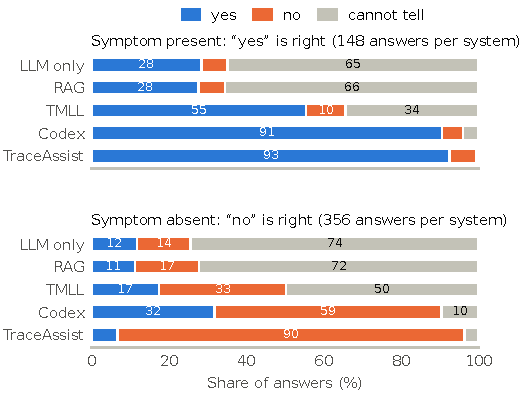
\includegraphics[width=\columnwidth]{verdicts}
\Description{Two panels of horizontal stacked bars, one per system, showing the share of yes, no and cannot-tell answers on present and on absent pairs.}
\caption{What each system answered (run 1, both wordings), as a share of its answers on pairs where the symptom is present (top) and absent (bottom). The text baselines mostly answer ``cannot tell''; TMLL and Codex commit more often, but raise more false alarms (``yes'' on absent pairs).}
\label{fig:verdicts}
\end{figure}

Fig.~\ref{fig:verdicts} shows what lies behind these numbers. The specificity of the text and TMLL baselines (0.83--0.89) looks close to \sysname's (0.93), but it is largely abstention. LLM only and RAG answered ``cannot tell'' to 72\% and 70\% of questions, which counts as a true negative on an absent pair; when they did answer ``yes'', half of their answers were wrong (precision 0.50 and 0.51). TMLL abstained less (45\%) and found more (recall 0.55), but raised 62 false alarms, two and a half times as many as \sysname. \sysname abstained on 3\% of answers and was right on 85\% of its ``yes'' answers. On the 12 answers where the trace cannot show the symptom, it answered ``cannot tell'' every time; the baselines did so 10--11 times, mostly as part of their general abstention. Codex rarely abstained (8\%) and raised the most false alarms of any system, 113, nearly five times \sysname's; 76 of them came from the everyday wording, where its specificity fell from 0.79 to 0.57. An agent that measures something can almost always find a thread that waited or a call that was slow; deciding whether that is the problem the user asked about is the hard part.

\begin{table}[t]
\centering
\caption{Balanced accuracy by symptom group, question category, hub scope and wording (run 1). LLM: LLM only.}
\label{tab:breakdown}
\footnotesize
\setlength{\tabcolsep}{3.5pt}
\begin{tabular}{@{}lrrrrrr@{}}
\toprule
 & $n$ & LLM & RAG & TMLL & Codex & \sysname \\
\midrule
Timing           & 62  & .57 & .56 & .64 & .75 & .98 \\
Waiting          & 152 & .56 & .57 & .63 & .77 & .87 \\
CPU              & 122 & .60 & .60 & .85 & .88 & .94 \\
Syscalls and I/O & 54  & .77 & .72 & .53 & .76 & .95 \\
Lifecycle        & 38  & .53 & .62 & .79 & .87 & .90 \\
Pipelines        & 36  & .49 & .43 & .78 & .91 & 1.00 \\
Unexpected       & 40  & .60 & .58 & .58 & .58 & .96 \\
\midrule
Comprehension    & 102 & .57 & .60 & .75 & .82 & .96 \\
Root cause       & 116 & .48 & .52 & .72 & .75 & .94 \\
Dependency       & 96  & .61 & .59 & .59 & .83 & .86 \\
Quantitative     & 126 & .61 & .60 & .71 & .78 & .93 \\
Remediation      & 64  & .73 & .68 & .66 & .85 & .98 \\
\midrule
Single-hub       & 228 & .64 & .62 & .64 & .77 & .92 \\
Multi-hub        & 276 & .52 & .54 & .74 & .81 & .94 \\
\midrule
Precise wording  & 252 & .58 & .56 & .68 & .84 & .96 \\
Everyday wording & 252 & .59 & .60 & .70 & .75 & .90 \\
\bottomrule
\end{tabular}
\end{table}

\subsection{RQ3: Where Systems Fail}

Table~\ref{tab:breakdown} breaks the results down. \sysname scores at least 0.86 in every row. Its weakest group is \emph{waiting} (0.87), which holds 12 of its 24 false positives and 7 of its 11 false negatives. Most of these come from symptoms that a kernel trace shows only indirectly. A convoy, a lock holder blocking others, and lock contention all appear as futex waits; the trace does not record which thread owns a lock, so they are inferred from wake-ups, and \sysname confused them on \texttt{batch\_server}'s traces, including its healthy run. \texttt{kvstore}'s slow backend was missed in both wordings: its clients are woken through loopback networking, so the critical path ends at ``network'' instead of reaching the server process.

The baselines fail differently. Multi-hub questions, which need evidence from several threads, are where the trace-text baselines are weakest (0.52 and 0.54 against 0.64 and 0.62 single-hub), as in our earlier study and in TAAF~\cite{ezaz2026taaf}: a few milliseconds of events rarely show a chain of waits. Root-cause questions are the hardest for them (0.48 and 0.52). TMLL is strong where its standard analyses match the symptom, on CPU symptoms (0.85), and weak on system calls and I/O (0.53), where an answer needs to know which file or call a thread used, which its standard analyses do not report. Codex is strongest on pipeline, CPU and lifecycle symptoms (0.87--0.91) and weakest on unexpected behaviour (0.58), where it called normal activity unexpected on 21 of 28 absent pairs.

\textbf{Wording.} The everyday wording costs \sysname 0.06 (0.96 to 0.90): 18 of its 24 false positives come from it, typically when a vague ``too long'' meets a normal-sized effect. Its two wordings disagree on 40 of 258 pairs. The baselines' verdicts depend more on wording: they disagree on 92--102 pairs, and the vaguer wording makes LLM only and RAG \emph{less} cautious (abstention falls from 81--83\% to 57--63\%) and more often wrong (specificity falls from 0.96--0.97 to 0.80--0.81).

\subsection{RQ4: Consistency}

Across \sysname's three runs, balanced accuracy is $0.930 \pm 0.005$. 474 of the 516 answers (92\%) got the same verdict all three times; 457 were right every time and 24 wrong every time. The persistent errors are systematic rather than chance: 11 are on \texttt{batch\_server}, mostly its lock symptoms confused with one another, 3 are barrier-straggler false alarms on \texttt{crunch}, and the rest include the loopback blind spot. The 42 answers that vary between runs are spread over both wordings (24 everyday, 18 precise); 17 of them concern waiting symptoms.

\subsection{RQ5: Cost and Time}

\begin{figure}[t]
\centering
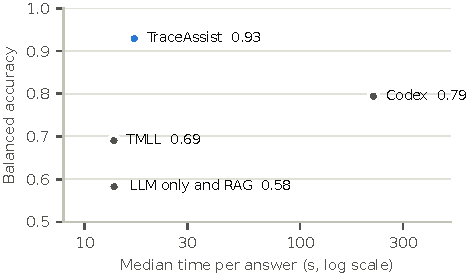
\includegraphics[width=\columnwidth]{time_accuracy}
\Description{Scatter plot of median seconds per answer against balanced accuracy: TraceAssist at 17 s and 0.93, Codex at 219 s and 0.79, TMLL at 14 s and 0.69, LLM only and RAG at 14 s and 0.58.}
\caption{Median time per answer against balanced accuracy (run 1). Times are wall-clock per answer, as recorded by each system's runner; TraceAssist's include building Trace Compass's analyses on the first question about each trace.}
\label{fig:time}
\end{figure}

Fig.~\ref{fig:time} relates time to accuracy.
\sysname's median answer took 17\,s on a desktop workstation; the first question on each trace, which also builds Trace Compass's analyses, took a median of 30\,s. Its answer call used about 27{,}000 input tokens, against 160{,}000--205{,}000 for the LLM-only, RAG and TMLL baselines, because it sends computed findings instead of trace text or every analysis; those baselines answered in a median of 14\,s. \sysname's answer calls cost \$1.41 for all 516 answers; the skills' calls were not logged, so its full cost is somewhat higher. Codex took a median of 219\,s per answer, 13 times \sysname's, running a median of 16 shell commands (11--25 for the middle 80\%) and reading an average of 0.69 million input tokens per answer (92\% from the prompt cache); its 516 answers cost \$9.50. A full bench run of \sysname, asking one question at a time, takes about 3 hours; the LLM-only, RAG and TMLL baselines took 1.2--1.3 hours each (plus 1.3 hours to collect TMLL's evidence), and Codex 17.7 hours with two sessions in parallel.

\subsection{Lessons Learned}
\label{sec:lessons}

We built \sysname against the bench, and each of the fixes below answered a failure the bench exposed. Five lessons generalize beyond our system.

\textbf{1. Measure false alarms, not only answers.} Our prototype evaluation asked only questions whose answer was ``yes'', and \sysname answered all of them correctly. The bench showed that the same system said ``yes'' too often: in a healthy program some thread always finishes last and some wait is always the longest, and the answer writer reported them as problems. Adding sizes to findings (a bottleneck's share of the round, counts of delays by length) and a rule that the answer weigh them against the question's threshold, together with explicit thresholds in the precise wordings, removed most of these false alarms. Negative controls are cheap to build into a test program and are the only way to see this failure.

\textbf{2. Absence of an event is evidence too.} \sysname first answered ``no'' to ``is batch\_server deadlocked?'' on a deadlocked trace. The execution graph records a wait when the thread is woken; a thread that is never woken leaves no wait, so every wait-chain analysis skipped the deadlock. Stuck-wait detection, which reads what each thread is still blocked in at the end of the trace, fixed the hang, deadlock and never-exit cases. The test harness had the same blind spot in reverse: its watchdog's exit woke the blocked threads inside the trace, and the critical path blamed the watchdog.

\textbf{3. Optional evidence fails silently.} \sysname still answers when TMLL is unavailable, only with less evidence. For part of development, every bench answer lacked TMLL's evidence, because its service failed whenever the trace was not open in the Trace Server. Later, a stale experiment index made TMLL allocate 23\,GB and be killed. Neither raised an error in the answers. We now check the services' health around every answer and stamp each answer with a fingerprint of the build and knowledge base, so results from different versions never mix.

\textbf{4. Documentation can leak the answer.} Our first knowledge base, like our prototype's, included a description of \texttt{batch\_server}, standing in for an organization's internal documentation. It named the threads and the lock, and answers cited it instead of the trace. We removed it before the three runs reported here, so their answers rest on the trace alone. Program documentation is valuable in deployment, but an evaluation must separate what the trace shows from what the documents say.

\textbf{5. Put the model where language is needed.} Each LLM call in \sysname makes one narrow decision whose output code checks, and all facts come from code. This kept a small, cheap model usable: the answer writer and two of the three skills run on \texttt{gpt-6-luna}. An agent that computes its own evidence, Codex, took 13 times as long per answer and raised nearly five times as many false alarms (113 against 24).

% 7 Threats to validity and open problems -- 0.6 page
\section{Threats to Validity and Open Problems}
\label{sec:threats}

\textbf{Internal validity.} We developed \sysname against the bench, so it may fit the bench better than unseen problems. Three things limit this: the answer keys come from the programs' fault switches, not from \sysname; the question thresholds were set by measuring every trace before \sysname's final runs; and the configuration used here was frozen and fingerprinted before them. Still, the fixes in Section~\ref{sec:lessons} were found on these traces, and the baselines received no such tuning. \sysname's thread\_finder uses a larger model than the baselines, which all use \texttt{gpt-6-luna}; the answer itself is written by the same model in every system. The baselines ran once each, for cost; \sysname's run-to-run spread ($\pm$0.005) suggests one run is representative for an LLM pipeline of this kind, but we did not measure theirs.

\textbf{External validity.} The programs are small and inject one fault at a time, whereas real systems often have several problems together and far more threads. All traces come from one machine and kernel and last 30\,s; our earlier prototype handled traces of up to 30 minutes, but not on this bench. All systems used one model family. The knowledge base includes 10 off-topic Django documents, which act as distractors, and no program documentation.

\textbf{Construct validity.} Verdicts are read from one line, so an answer that names the wrong thread still counts as a true positive. The bench includes an answer key with the threads, causes and numbers a correct answer should give; grading answers against it is future work.

\textbf{Open problems.} Several symptoms are hard to see in a kernel trace. Memory pressure needs page-fault and kernel-memory events that our kernel's LTTng lacks. Busy-waiting looks the same as computing. A trace does not record lock owners, so convoys and lock contention are inferred, and these caused the largest share of \sysname's persistent errors. Wake-ups through loopback networking end the critical path at ``network'' instead of the peer process. The critical path also stops at preemption: it shows that a thread on the path waited for a CPU, but not which thread held it, so on a priority inversion an answer can report the holder's 15\,ms wait for a CPU in every round without naming the real-time thread that preempted it. Beyond detection, production use raises questions this bench does not answer: traces from many hosts, user-space and kernel events together, and the cost of the thread search on systems with thousands of threads.

% 8 Conclusion -- 0.35 page (with data availability)
\section{Conclusion}

Execution traces are too large for an LLM to read and describe executions it has never seen. \sysname, developed for Ciena, answers questions about Linux kernel traces by having Trace Compass compute the evidence from the whole trace, using the LLM only for small checked decisions and for writing the answer from that evidence. On a bench of nine fault-switch programs that asks every question of traces with and without its symptom, it reached a balanced accuracy of 0.93, against 0.58--0.79 for four baselines using the same answering model, and it rarely reported problems that were not there. Developing against negative controls exposed failures that a question set with only ``yes'' answers had hidden. Next steps are grading the content of answers against the bench's answer keys, inferring lock ownership, following wake-ups across loopback networking, and evaluating \sysname on traces from Ciena's systems.

\paragraph{Data availability.} We will release the bench's traces, the 112 questions, and every system's answer and verdict for each question upon publication.


\begin{acks}
% Confirm with the professor that this work was funded through Mitacs, and add
% the grant number if there is one (e.g. "through Mitacs Accelerate grant IT...").
We thank Ciena for their collaboration and Mitacs for their support.
% Same disclosure as the CASCON draft; update to match what actually applies.
Text drafted and edited with the assistance of Claude Code (Anthropic,
Claude Opus), with additional text editing by Codex (OpenAI); the authors
designed the experiments, collected and analyzed all data, and verified
all content.
\end{acks}

\bibliographystyle{ACM-Reference-Format}
\bibliography{references}
\end{document}
